Dies ist die Anleitung für die Benutzung des School Information Service der HTL Anichstraße. Diese Anleitung wurde im Zuge der Diplomarbeit vom SIS-Team geschrieben, um alle Funktionen unseres Systems zu dokumentieren.

\section{Allgemein}
Nach der Anmeldung mit Benutzerdaten (dieselben wie bei moodle oder htl-wlan, siehe (\autoref{fig:Web_Login}) erscheint das Frontend (\autoref{fig:Web_Access}). \\

\begin{figure}[H]
\centering
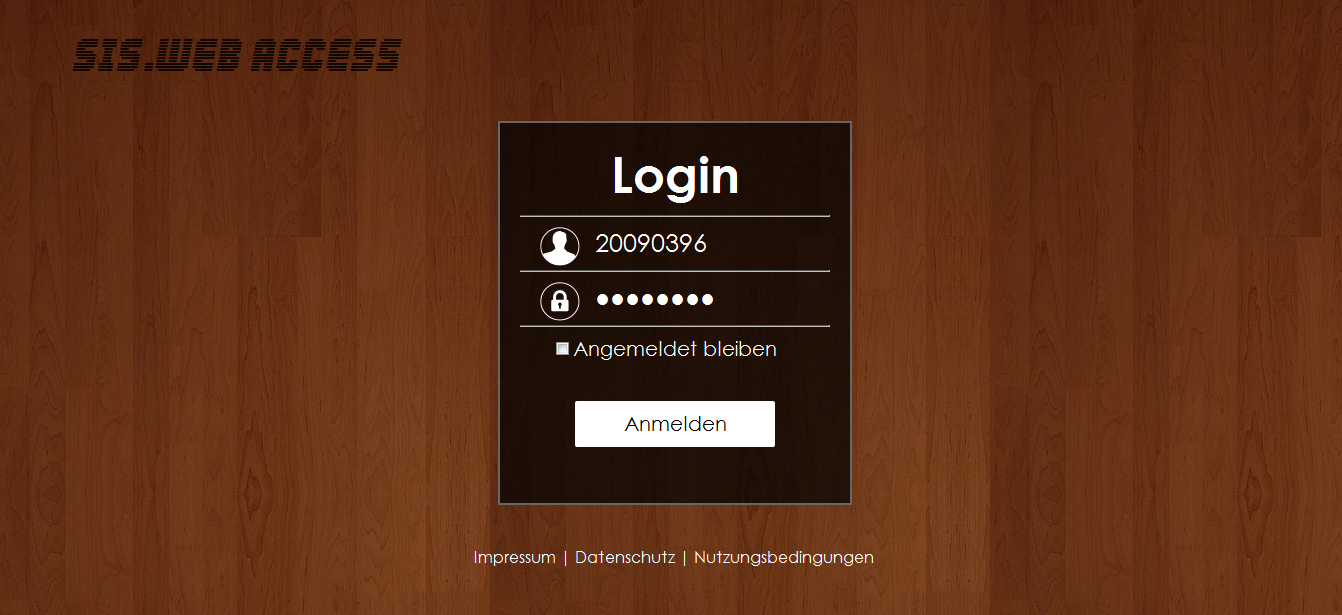
\includegraphics[keepaspectratio=true, width=14cm]{images/screenshots/login.png}
\caption{Web-Loginbereich}
\label{fig:Web_Login}
\end{figure}

\begin{figure}[H]
\centering
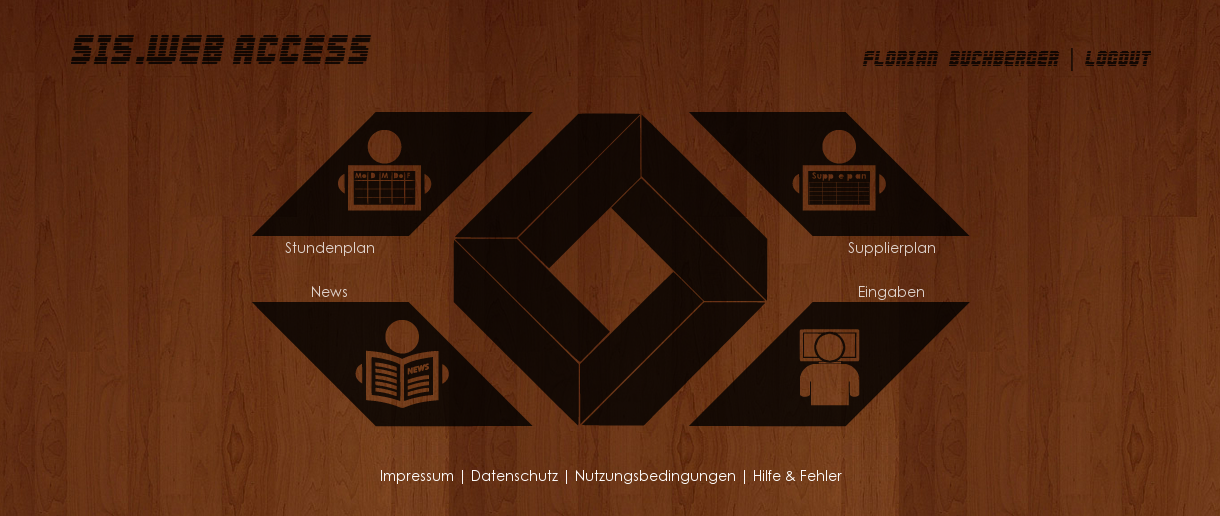
\includegraphics[keepaspectratio=true, width=14cm]{images/screenshots/web-access_nohover.png}
\caption{Web-Frontend}
\label{fig:Web_Access}
\end{figure}

Durch einen Klick auf eines der Symbole schiebt sich, bei aktiviertem JavaScript, die Seite auseinander und der Inhalt wird angezeigt. Um zum Menü zurückzukehren kann  das Kreuz rechts oben verwendet werden. Ein Klick auf den oberen oder unteren Rand der Seite hat den gleichen Effekt.\\
Durch einen Klick auf die Schrift im linken oberen Eck oder auf das SIS-Logo in der Mitte gelangt man zum übergeordneten Menü zurück.\\
Um sich abzumelden muss \enquote{LOGOUT} in der rechten oberen Ecke angeklickt werden.\\
Ein Icon, das zwar angezeigt wird, jedoch nicht anwählbar ist, ist auf eine mangelnde Berechtigungsstufe zurückzuführen.\\
Durch Auswählen von \enquote{Fehler} wird ein Fenster geöffnet, mit dem eine E-Mail an das SIS-Team gesendet werden kann, um Fehler zu melden.\\
Zudem ist diese Anleitung unter dem Punkt Hilfe abrufbar.